\documentclass{article}
\usepackage[utf8]{inputenc}
\usepackage[T1]{fontenc} 
\PassOptionsToPackage{hyphens}{url}\usepackage[hidelinks]{hyperref}
%\usepackage[french]{babel}
\usepackage{charter} 
\usepackage{graphicx} 
\usepackage{amsmath}
\usepackage{amsthm}
\usepackage{amsfonts}
\usepackage{geometry}
\usepackage{cancel}
\usepackage{enumerate}
\usepackage{stmaryrd}
\usepackage{mathrsfs}
\usepackage{amssymb}
\geometry{hmargin=2.7cm,vmargin=2.5cm}

\usepackage{color}
\usepackage{listings}

\definecolor{dkgreen}{rgb}{0,0.6,0}
\definecolor{gray}{rgb}{0.5,0.5,0.5}
\definecolor{mauve}{rgb}{0.58,0,0.82}

\lstset{
  frame=single,
  language=C++,
%   aboveskip=3mm,
%   belowskip=3mm,
  showstringspaces=false,
  columns=flexible,
  basicstyle={\ttfamily},
  numbers=none,
  numberstyle=\tiny\color{gray},
  keywordstyle=\color{blue},
  commentstyle=\color{dkgreen},
  stringstyle=\color{mauve},
  breaklines=true,
  breakatwhitespace=true,
  tabsize=3
}

\usepackage{footnote}

\usepackage{multirow}
\newcommand{\specialcell}[2][c]{%
  \begin{tabular}[#1]{@{}c@{}}#2\end{tabular}}

\usepackage{lastpage}
\usepackage{fancyhdr}
\pagestyle{fancy}
\renewcommand{\headrulewidth}{0pt}
\renewcommand{\footrulewidth}{0.5pt}
\fancyhead[L]{}
\fancyhead[R]{}
\fancyfoot{}
\fancyfoot[L]{RS -- Quentin CHAN-WAI-NAM}
\fancyfoot[R]{\thepage/\pageref{LastPage}}

\fancypagestyle{plain}{
	\renewcommand{\headrulewidth}{0pt}
	\renewcommand{\footrulewidth}{0.5pt}
	\fancyhead[L]{}
	\fancyhead[R]{}
	\fancyfoot{}
	\fancyfoot[L]{RS -- Quentin CHAN-WAI-NAM}
	\fancyfoot[R]{\thepage/\pageref{LastPage}}
}

\usepackage{animate}

% \def\thesubsection{\thesection.\alph{subsection}}

\makeatletter
\def\thm@space@setup{%
  \thm@preskip=15pt \thm@postskip=15pt
}
\makeatother

\linespread{1.3}

\newcommand{\abs} [1] {\left| #1 \right|}
\newcommand{\scal}[2]{\left\langle #1 , #2 \right\rangle}
\newcommand{\dif}[0]{\text{\:d}}
\newcommand{\Dpar}[2]{\frac{\partial#1}{\partial#2}}

\newcommand{\ceil}[1]{\lceil#1\rceil}
\newcommand{\floor}[1]{\lfloor#1\rfloor}

\newcommand{\Four}[1]{\widehat{#1}}

\newcommand{\norm}[1]{\left\lVert#1\right\rVert}

\newcommand{\petito}[1]{o\mathopen{}\left(#1\right)}
\newcommand{\grandO}[1]{O\mathopen{}\left(#1\right)}

\def\R{\mathbb{R}}
\def\Z{\mathbb{Z}}
\def\N{\mathbb{N}}
\def\e{\text{e}}
\def\d{\text{d}}
\def\Re{\text{Re}}

\def\Per{\text{Per}\,}
\def\Ker{\text{Ker}\,}
\def\Im{\text{Im}\,}

\def\Ind{\mathbf{1}}

% Width of the EPIs
\def\epiWidth{0.7}
\def\cropcHeight{2.93cm}

\newcommand{\Binom}[2]{\begin{pmatrix} #1 \\ #2 \end{pmatrix}}

\newcommand{\vect}[1]{\mathbf{#1}}

%%%%%%%%%%%%%%%%%%%%%%%%%%%%%%%%%%%%%%%%%%%%%%%%%%%%%%%%%%%%%%%%%%%%%%%%%%%%%%%%%%%%%%%%%%%%%%%%

\title{RS: Epipolar Plane Image Analysis\\Application to SkySat videos}
\date{\today}
\author{Quentin CHAN-WAI-NAM}

\theoremstyle{definition}
\newtheorem{question}{}

\begin{document}
\maketitle

\begin{center} Supervised by Gabriele FACCIOLO and Andrés ALMANSA. \end{center}

\begin{abstract}
This document describes and implements a depth estimation method using ``light fields'', i.e. dense sets of images captured along a linear path, based on a method originally presented by Kim et al. in \cite{art:kim13:lfields}. We test the proposed approach in the context of satellite optical imaging.
\end{abstract}


\tableofcontents

\clearpage
\section{Description of the probem and setup}



\paragraph{Light fields} In \cite{art:kim13:lfields}, Kim et al. describe a method for computing precise and exhaustive depth maps using ``light fields'', i.e. dense sets of images captured along a linear path. By concatenating one line of the rectified images together, one obtains an ``epipolar-plane image'' (EPI), in which a single scene point appears as a linear trace which slope depends directly on its distance to the camera. Thus, by estimating these slopes, one can reconstruct the disparity of each point of the scene. Using camera parameters, one can then reconstruct the depth of each point from the measured disparity. This is summarized in Figure \ref{drawing:light_fields}.


\begin{figure}[ht]
\centering
 \includegraphics[width=0.6\textwidth, trim=2cm 8cm 2cm 3cm, clip]{drawings/light_fields.eps}
 \caption{Light field capture process. Top: a camera captures the scene along a linear path. Middle: by concatenating the images, one obtains a pile of images with spatial dimensions $(v, u)$ and temporal dimension $s$. Bottom: by slicing along a single row $v$ (in red), one obtains an EPI (epipolar-plane image, along dimensions $(s, u)$) in which single points in the scene create a linear trace.}
 \label{drawing:light_fields}
\end{figure}


Some real examples of EPIs are presented in Figure \ref{fig:exepi}. Compared to using only pairs of images, proceeding with light fields for stereo reconstruction could enable more precise depth estimations and natural ways to handle occlusions (since an object might be occluded only on some frames and not others). Compared to direct 3D point acquisition using 3D scanners, the method should prove faster (one only has to capture the images and may leave the computation of the actual depth map for later) and more resilient to occlusions for instance (since the camera viewpoint changes, the occlusions may also change). A downside of this method is that it proves computationally expensive. This initially limits its application to low resolution images. The method presented by \cite{art:kim13:lfields} tackle this particular issue.


The authors use very high definition images -- the article thus describe several implementation details in order to ensure computational feasibility, both in terms of space (sparse representation of light fields) and computational power. For instance, they prefer local optimization near object boundaries and propagation to nearby areas in a fine-to-coarse approach to global optimization on the whole image. In the end, the method seems relatively fast, precise and robust to inconsistencies and outliers.


\paragraph{Goal} The goal of this project is to adapt the method proposed by Kim and al., that they tested on urban landscapes with mainstream cameras, to the context of satellite images. It should noted that the case of rectified satellite images correspond to case of a set of images taken along a linear path. The images are registered in such a way that the ground doesn’t move. We chose not to focus on GPU implementation and memory management and choose to proceed with mildly high resolution images to ensure computational feasibility.


\begin{figure}[t]
  \centering
  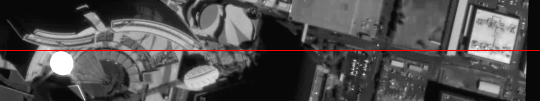
\includegraphics[width=\epiWidth\textwidth]{images/1519991772641_1st.png}\\
  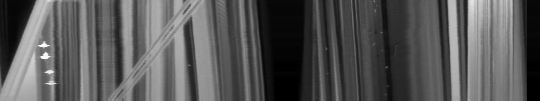
\includegraphics[width=\epiWidth\textwidth]{images/1519991772641_epi.png}\\[0.5cm]
  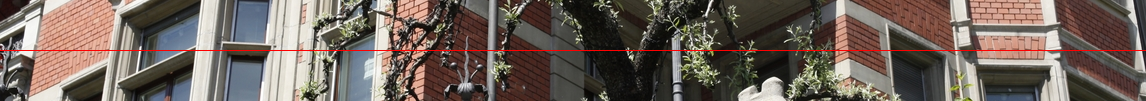
\includegraphics[width=\epiWidth\textwidth]{images/1521725699383_1st.png}\\
  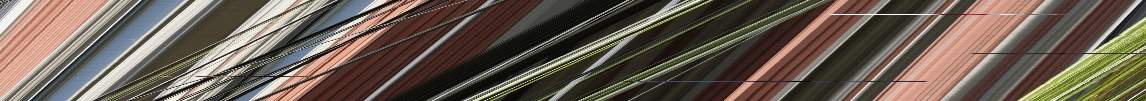
\includegraphics[width=\epiWidth\textwidth]{images/1521725699383_epi.png}
  \caption{Sample EPIs from SkysatLR18 (top) and MansionLR (bottom) datasets. We see that individual points leave a linear trace in the temporal dimension and that occlusions change over time.}
  \label{fig:exepi}
\end{figure}


\section{Description of the method}


\subsection{Disparity estimation from EPIs on confident points}


\paragraph{Principle} The main idea is, given a list of candidate disparities, to select the best slope for each point at which a confident measure can be done. Given a single line of an EPI, one first computes a confidence score. Then, for each confident point, one select the slope such that pixel radiances on the resulting line are the most densely distributed around a given mean radiance. This process is robust to occlusions.


\paragraph{Details} Let us consider some EPI $E$ corresponding to a fixed $v$, which dimensions are $s$ along the rows and $u$ along the columns. We work only on one line of this EPI at a time (beginning with the center line at $\widehat{s} = s_{\max} / 2$).



\begin{figure}[ht]
\centering
 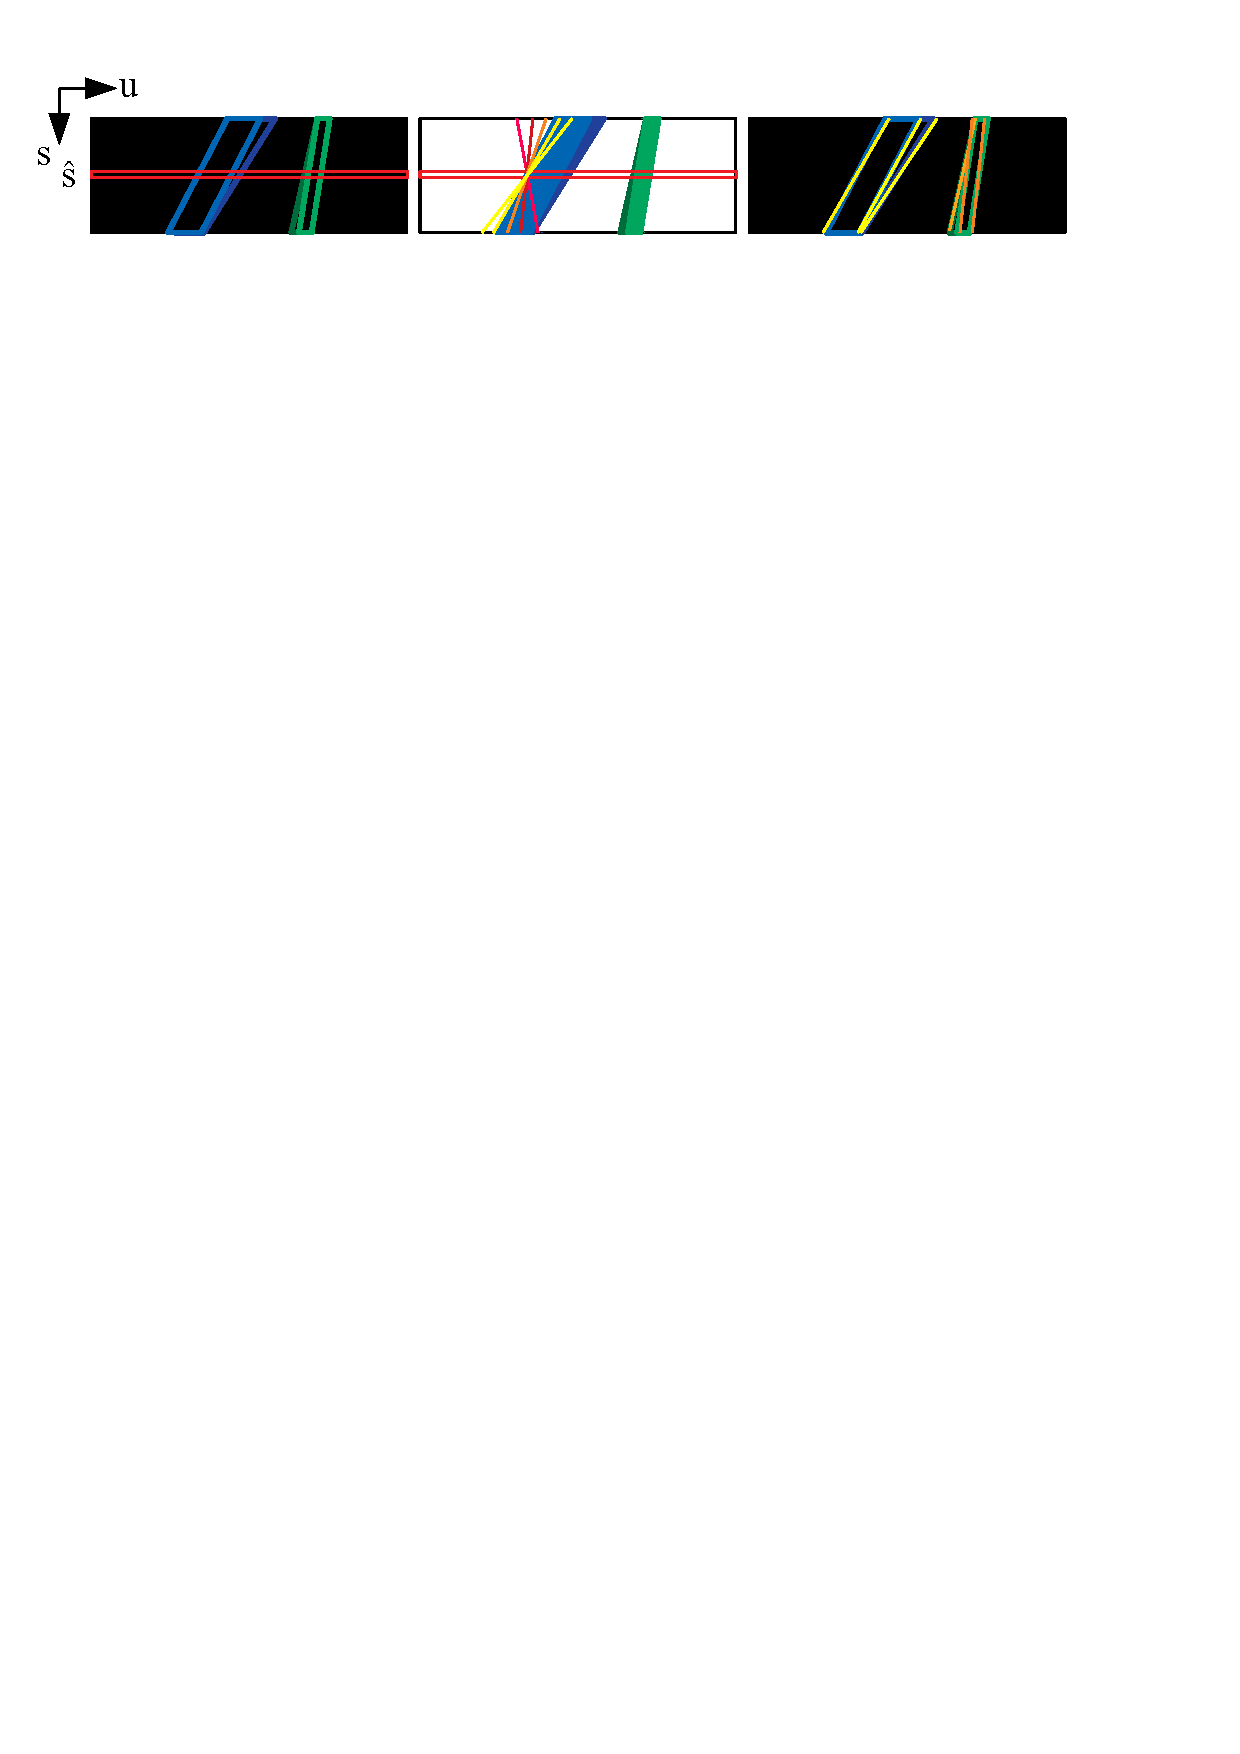
\includegraphics[width=1.0\textwidth, trim=0.5cm 25.5cm 2.5cm 1cm, clip]{drawings/depth_estimation.pdf}
 \caption{Disparity estimation process. Left: we select a row $\widehat{s}$. Middle: given a column $u$, we test several candidate $d$'s and select the one with the highest score $S(u, d)$. Right: we propagate the disparity along the temporal dimension for points belonging to  a confident edge, then repeat the process along each column $u$, and for every value $\widehat{s}$ if $d(\widehat{s}, u)$ was not computed yet.}
 \label{drawing:depth_estimation}
\end{figure}



To each point, we define an edge confidence measure $C_e$ such that
\begin{align}
 C_e (\widehat{s}, u) &= \sum_{u' \in \mathcal{N}_{C_e}(\widehat{s}, u)} \norm{E(\widehat{s}, u) - E(\widehat{s}, u')}^2. 
\end{align}
This measures diversity in the radiances of the image along a small linear window $\mathcal{N}_{C_e}(\widehat{s}, u)$ around the point $(\widehat{s}, u)$. It should be high on edges that show great color transitions and low on flat surfaces. The process is illustrated in Figure \ref{drawing:fine_to_coarse}.


The disparity estimation process is detailed in Figure \ref{drawing:depth_estimation}. Let $d_\text{list} = \left\{d_1, \cdots, d_D \right\}$ be a set of candidate disparities. We compute the set of radiances $\mathcal{R}$ of values of $E$ along the line centered on $u$ of slope $d$, for all confident couples $(u, d)$, i.e. at points $(\widehat{s}, u)$ such that $C_e(\widehat{s}, u) > \varepsilon_{C_e}$:
\begin{align} 
\mathcal{R}(u, d) &= \left\{ E(u + (\widehat{s} - s) d, s) \; | \; s = 0 \cdots S-1 \right\}.
\end{align}

We then select the $d$ with the best score $S(u, d)$ defined as:
\begin{align} 
S(u, d) = \frac{1}{\abs{\mathcal{R}(u, d)}} \sum_{\mathbf{r} \in \mathcal{R}(u, d)} K(\mathbf{r} - \overline{\mathbf{r}})
\end{align}
where $\mathbf{r}$ is a value $E(\cdot, \cdot)$, $\overline{\mathbf{r}}$ is some mean radiance value described hereafter, and $K$ is a ``kernel''. We choose the kernel presented in the article, i.e.
\begin{align}
K(\mathbf{r}) = \left\{ 
\begin{array}{l}
1 - \norm{\mathbf{r} / h}^2 \qquad \text{if $\norm{\mathbf{r} / h} < 1$} \\
0 \qquad \text{else}                            
\end{array} \right. .
\end{align}
We name this kernel the ``bandwidth kernel'' (where $h$ is a parameter). Its value is $0$ when $\norm{\mathbf{r}} \rightarrow +\infty$ and $1$ for $\norm{\mathbf{r}} \rightarrow 0$. Its role is to select $\mathbf{r}$ values that are reasonably near zero.

$\overline{\mathbf{r}}$ is a parameter that depends on $(u, d)$: following the article, we perform a truncated mean-shift algorithm (10 iterations), with $\overline{\mathbf{r}}_0 = E(u, \widehat{s})$ and
\begin{align} 
\overline{\mathbf{r}} \leftarrow \frac{\sum_{\mathbf{r} \in \mathcal{R}(u, d)} K(\mathbf{r} - \overline{\mathbf{r}}) \mathbf{r}}{\sum_{\mathbf{r} \in \mathcal{R}(u, d)} K(\mathbf{r} - \overline{\mathbf{r}})}
\end{align}
prior to the computation of $S(u, d)$, initializing with $\overline{\mathbf{r}} = E(\widehat{s}, u)$. The expected result is that $\overline{\mathbf{r}}$ will shift to the mean of the closest blob of radiances near $E(\widehat{s}, u)$, ignoring the values that are too far from this value (that are expected to be occlusions).


\paragraph{Technical difficulties} A line defined by $(u + (\widehat{s} - s) d, s)$ will very certainly have non-integer coordinates or go out of the image boundaries. We thus take the following decisions:
\begin{itemize}
 \item Values outside of the image are considered \emph{nan} and not taken into account in $\mathcal{R}(u, d)$.
 \item We have yet to decide on some proper interpolation method for computing non-integer values of $E$, for instance linear interpolation along the line $E(u, \cdot)$.
\end{itemize}


\subsection{Selective median filtering}


We repeat the process for all the lines $v$ -- since the process is independent for each $v$, this operation can be simultaneous. When all lines $v$ have been computed, we apply a median filter on the resulting disparity map along dimensions $(v, u)$ such that in the end, for a point $(v, u)$ such that $C_e (v, u) > \varepsilon_{C_e}$, the selected value $d_{v, u}$ is the median value of the set:
\[ \left\{ d (v', u') \; | \; (v', u') \in \mathcal{N}_\text{sel. median}(v, u), \; C_e(v', u') > \varepsilon_{C_e}, \; \norm{E_{v}(\widehat{s}, u) - E_{v'}(\widehat{s}, u')} < \varepsilon_{E} \right\}.\]

$\mathcal{N}_\text{sel. median}(v, u)$ is a neighbourhood of $(v, u)$. The expected result is to filter speckles among points of the same color that are also close one to the other. After this step, all the disparities have been computed and filtered in points $(s, v, u)$ such that $C_e(s, v, u)$ was high enough.



\subsection{Depth propagation along temporal axis}


For each $u$, we select the $d$ with the best score. We then propagate the disparities from $\widehat{s}$ to the other $(s', u')$ simply by drawing the depths along the lines $u' = u + (\widehat{s} - s)d$ if 
\begin{enumerate}
 \item $C_e(\widehat{s}, u) > \varepsilon_{C_e}$
 \item $C_e(s', u') > \varepsilon_{C_e}$
 \item $\norm{E(s', u') - E(\widehat{s}, u)} < \varepsilon_E$
\end{enumerate}
These points $(s', u')$ are marked as computed and not considered anymore. The algorithm then proceeds to new values $s$ that are close to $\widehat{s}$ (i.e. $s_{\max} / 2 + 1$, $s_{\max} / 2 - 1$, ...) and repeat the process.


After these steps, we obtain disparity values for each point such that $C_e$ was high enough, the other points having been masked.


\paragraph{Differences with the article} It should be noted that in \cite{art:kim13:lfields}, Kim et al. handle the situation in which a point with high edge confidence $C_e$ could have a bad disparity estimation $d$. This could for instance happen if the point is in the intersection of two lines of the same color with different slopes in the EPI. In order to do so, the authors define a disparity confidence score
\begin{align}
 C_d (\widehat{s}, u) &= C_e (\widehat{s}, u) \left|\max_d S(u, d) - \underset{d}{\mathrm{mean}}\, S(u, d)\right| \label{eq:c_d}
\end{align}
and only retain and propagate $d$'s corresponding to points with a high $C_d$. We chose not to use this conservative criterion since it decreases significantly the number of valid estimations and tend to erase mildly sharp borders on buildings in our satellite images, as shown in Section \ref{sec:results}.


\subsection{Fine-to-coarse approach}


The approach presented in \cite{art:kim13:lfields} is based on a ``fine to coarse'' approach. It consists in making confident disparity estimations in the images for different spatial scales $(v, u)$ and recombining these disparities in order to reconstruct a complete disparity map at the finest scale.


In order to proceed to a multi-scale analysis, the idea is to use the regularizing effect of downsampling. We thus create a pyramid of downsampled images, with coarser and coarser disparity estimations. The confident estimations at the finest scale are likely to be made on small objects or contours, whereas the estimations at the coarser scales will be related to plain surfaces for instance. The algorithm will then merge the estimations computed at the different scales by sequentially filling the blank estimations back from coarse to fine by upsampling disparity maps at a given scale to the preceding finer scale. This process is presented in Figure \ref{drawing:fine_to_coarse}.



\begin{figure}[ht]
\centering
 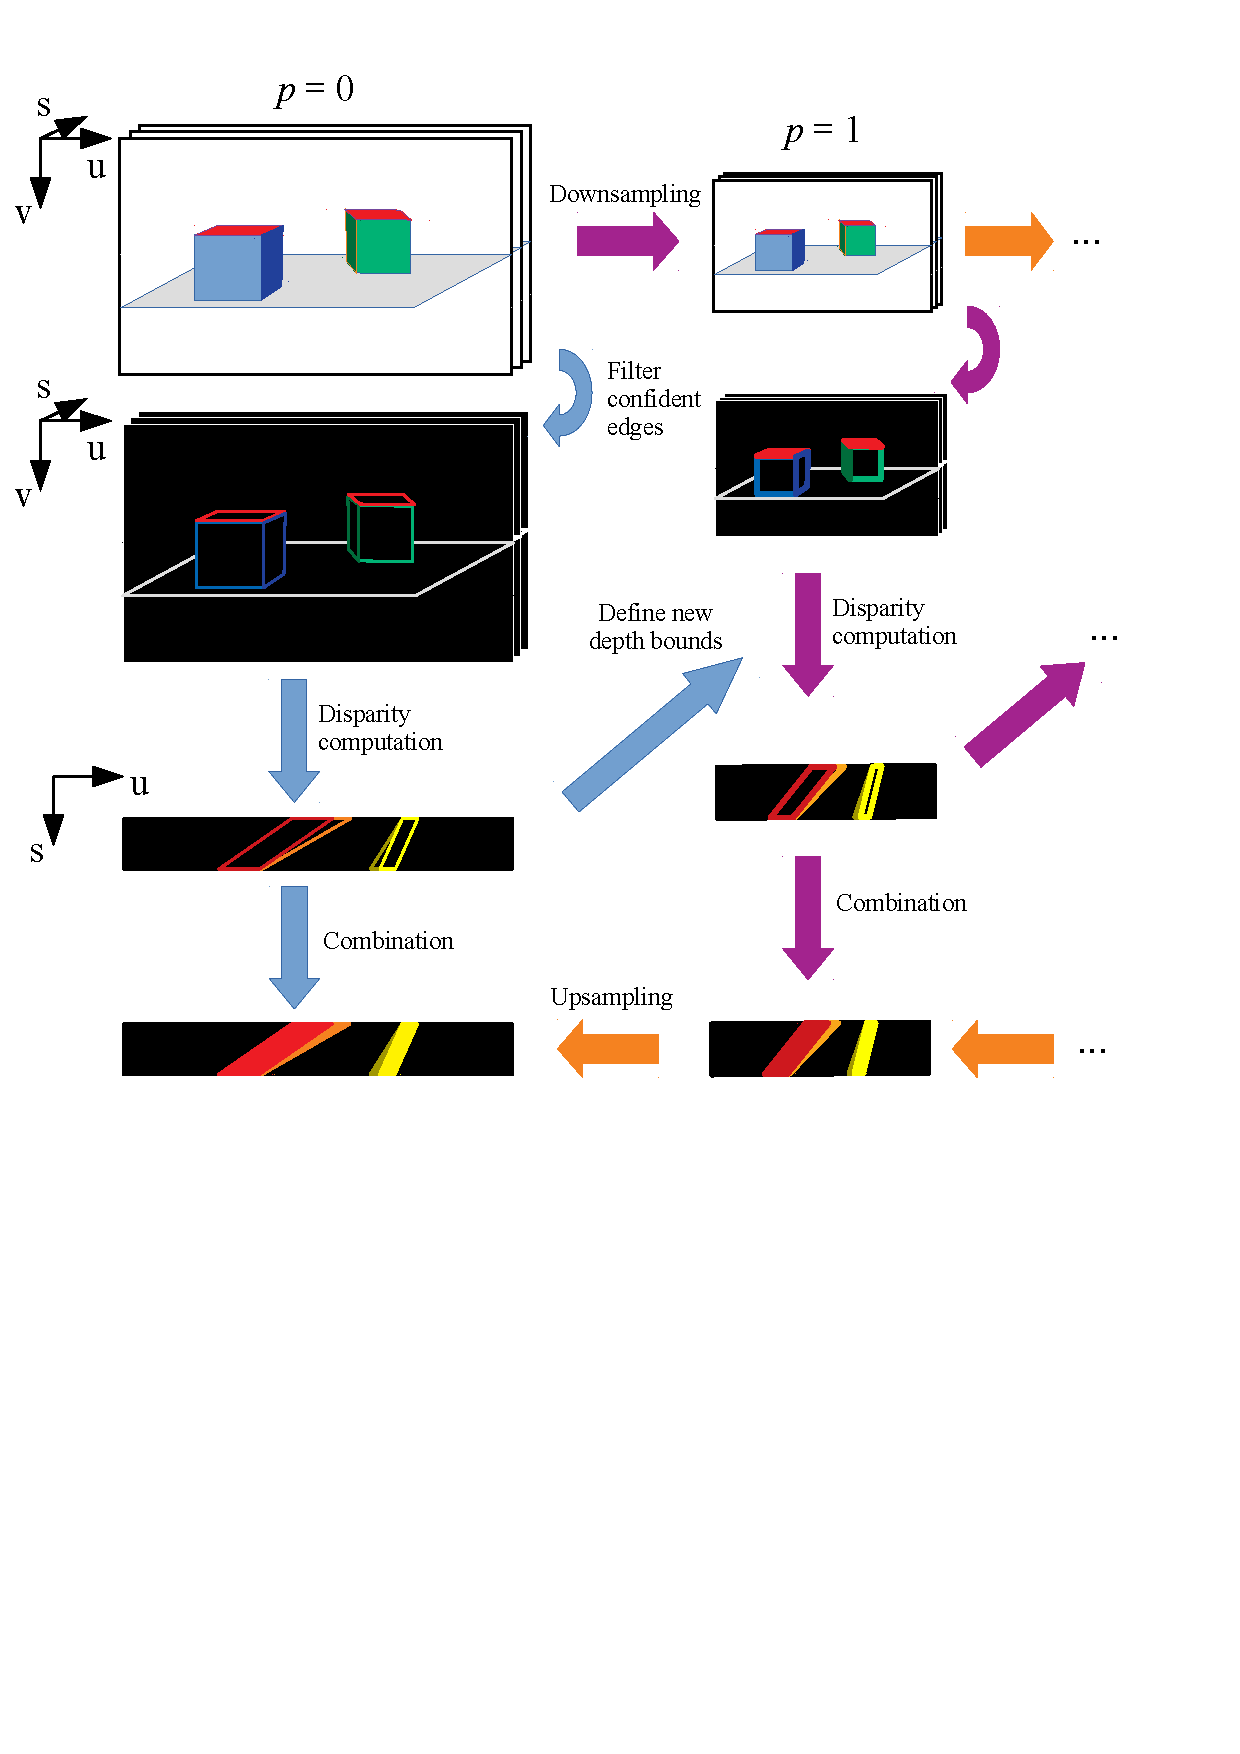
\includegraphics[width=1.0\textwidth, trim=0cm 11cm 0cm 0.5cm, clip]{drawings/fine_to_coarse.pdf}
 \caption{Fine to coarse approach.}
 \label{drawing:fine_to_coarse}
\end{figure}



\paragraph{Downsampling} We progressively fill the zones left blank by our confidence criterion (we choose here $C_e > \varepsilon_{C_e}$ ; one could apply $C_d > \varepsilon_{C_d}$ like in the article but this is significantly more conservative). This approach is similar to building a pyramid of images, and writes as follow:
\begin{enumerate}
 \item Let us consider a pile of images at the scale $p$ (the ``level $p$'' of the pyramid). One first applies a Gaussian filter in the spatial dimensions $(v, u)$ with window $\mathcal{N}_\text{downsampling}$.
 \item We then downsample the images by taking one line over 2 in the spatial dimensions $(v, u)$ ; the resolution along the temporal dimension $s$ is left unchanged. This is the scale $p+1$ of the pyramid of images.
 \item Then, we use the confident disparities computed at the scale $p$ in order to derive disparity bounds for the scale $p+1$. This step is not described precisely in the article ; we chose, given a point $(s, v', u')$ in $p+1$, to select the 2 pairs of points $(s, v, [u_1^1, u_2^1])$ $(s, v+1, [u_1^2, u_2^2])$ where $v = 2 v'$ and $u_1^1$, $u_1^2$ are the first confident points at the left and right of $u=2u'$. The bounds for $(s, v', u')$ will be the $\min$ and the $\max$ disparities among these points.
 \item We then perform a disparity computation along all axis as described in the preceding section.
\end{enumerate}
The pyramid process is represented in Figure \ref{fig:pyramid}. The confidence score will be less and less restrictive due to the regularization effect of downsampling.


\begin{figure}[th]
  \centering
  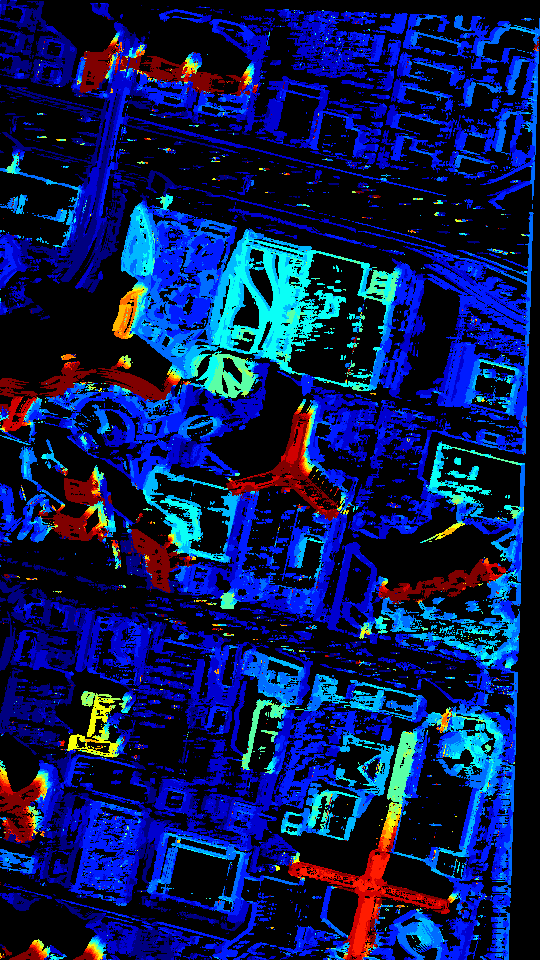
\includegraphics[width=0.4\textwidth]{images/pyr/1522269722500_pyr_depth_000.png}
  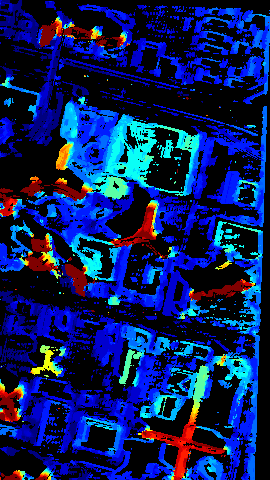
\includegraphics[width=0.2\textwidth]{images/pyr/1522269722500_pyr_depth_001.png}
  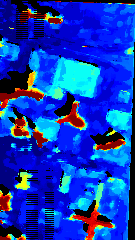
\includegraphics[width=0.1\textwidth]{images/pyr/1522269722500_pyr_depth_002.png}
  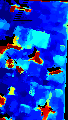
\includegraphics[width=0.05\textwidth]{images/pyr/1522269722500_pyr_depth_003.png}
  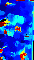
\includegraphics[width=0.025\textwidth]{images/pyr/1522269722500_pyr_depth_004.png}
  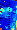
\includegraphics[width=0.0125\textwidth]{images/pyr/1522269722500_pyr_depth_005.png} \\
  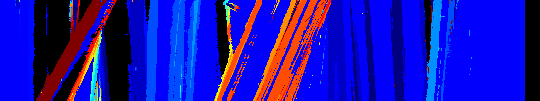
\includegraphics[width=0.4\textwidth]{images/pyr/1522269722500_pyr_epi_000.png}
  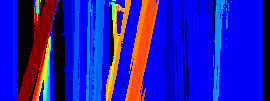
\includegraphics[width=0.2\textwidth]{images/pyr/1522269722500_pyr_epi_001.png}
  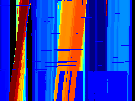
\includegraphics[width=0.1\textwidth]{images/pyr/1522269722500_pyr_epi_002.png}
  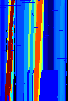
\includegraphics[width=0.05\textwidth]{images/pyr/1522269722500_pyr_epi_003.png}
  
\includegraphics[width=0.025\textwidth]{images/pyr/1522269722500_pyr_epi_004.png}
  
\includegraphics[width=0.0125\textwidth]{images/pyr/1522269722500_pyr_epi_005.png}
  \\[0.5cm]
  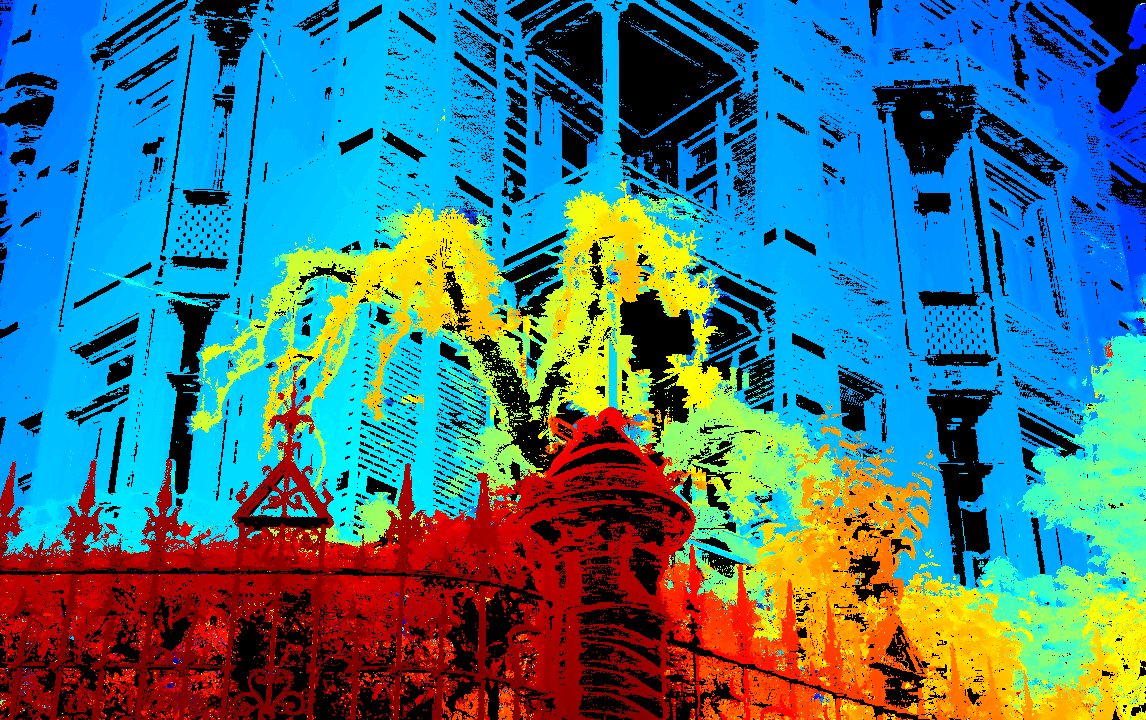
\includegraphics[width=0.4\textwidth]{images/pyr/1522286815730_pyr_depth_000.png}
  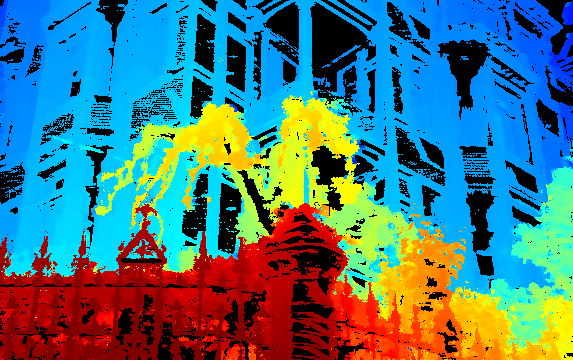
\includegraphics[width=0.2\textwidth]{images/pyr/1522286815730_pyr_depth_001.png}
  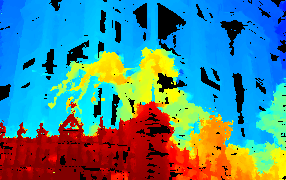
\includegraphics[width=0.1\textwidth]{images/pyr/1522286815730_pyr_depth_002.png}
  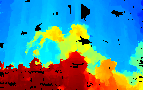
\includegraphics[width=0.05\textwidth]{images/pyr/1522286815730_pyr_depth_003.png}
  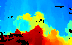
\includegraphics[width=0.025\textwidth]{images/pyr/1522286815730_pyr_depth_004.png}
  
\includegraphics[width=0.0125\textwidth]{images/pyr/1522286815730_pyr_depth_005.png}
  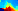
\includegraphics[width=0.00625\textwidth]{images/pyr/1522286815730_pyr_depth_006.png}\\
  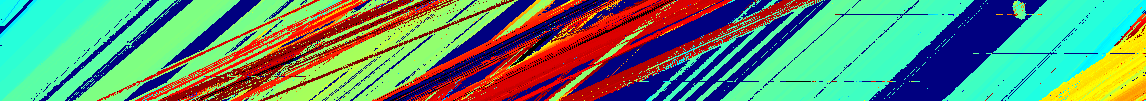
\includegraphics[width=0.4\textwidth]{images/pyr/1522286815730_pyr_epi_000.png}
  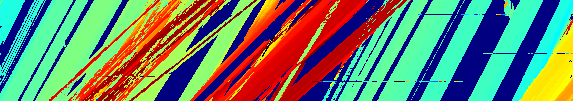
\includegraphics[width=0.2\textwidth]{images/pyr/1522286815730_pyr_epi_001.png}
  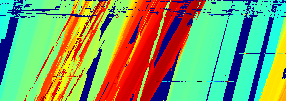
\includegraphics[width=0.1\textwidth]{images/pyr/1522286815730_pyr_epi_002.png}
  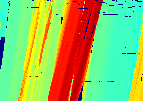
\includegraphics[width=0.05\textwidth]{images/pyr/1522286815730_pyr_epi_003.png}
  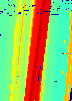
\includegraphics[width=0.025\textwidth]{images/pyr/1522286815730_pyr_epi_004.png}
  
\includegraphics[width=0.0125\textwidth]{images/pyr/1522286815730_pyr_epi_005.png}
  
\includegraphics[width=0.00625\textwidth]{images/pyr/1522286815730_pyr_epi_006.png}
  \caption{Pyramid of downsampled disparity maps and sample EPIs (after disparity computation) for the Skysat sequence with step 18 (SkysatLR18, top) and mansion sequence (MansionLR, bottom) with $240$ candidate values for $d$. Dark zones are either erased as shading or having a low edge confidence score $C_e$.}
  \label{fig:pyramid}
\end{figure}


\paragraph{Going back up to the finest scale} In order to retrieve the disparity map to the finest scale $p=0$, one then proceeds the other way round:
\begin{enumerate}
 \item Starting at $p=p_{\max}$, one upscales the disparity estimates (with bilinear interpolation) and the validity mask $M_e = \{C_e > \varepsilon_{C_e}\}$ (with nearest neighbour interpolation).
 \item Consider the disparity map at scale $p-1$. Fill the blank zones of this disparity map using the upscaled disparity map from $p$ at confident points from $M_e$.
\end{enumerate}


In the end, following the paper, we also make the following refinements:
\begin{itemize}
 \item We apply a median filter on the final disparity map estimates with window $\mathcal{N}_\text{fin. median}$.
 \item When establishing the map of valid points $M_e = \{C_e > \varepsilon_{C_e}\}$, one can perform a mathematical opening in order to remove falsely confident points. We find out that this degrades the performance of the algorithm on non-sharp images such as the Skysat sequence, so we chose to deactivate this feature.
\end{itemize}


\clearpage
\section{Results} \label{sec:results}


\subsection{Datasets and parameters} \label{subsec:dataset_params}


The parameters we used for the following results are presented in Table \ref{table:parameters}. We chose to test our algorithm on the original data of \cite{art:kim13:lfields} along with satellite images taken from a public Skysat video. The datasets are described in Table \ref{table:datasets}.


\paragraph{Parameters and number of channels} It should be noted that MansionLR is a RGB dataset and Skysat is a monochromatic dataset. Our kernels, confidence measure and color thresholds use the Euclidean norm of the values of images -- in order to use the same parameters for all the experiments and maintain coherence between the experiments, we decide to define the parameters for RGB images and redefine the Euclidean norm for the monochromatic images as follows:
\begin{align}
 \forall x \in \R, \qquad \norm{x} &= \sqrt{3} \times \abs{x}.
\end{align}
We could also redefine the norm for four-channel images for instance with a factor $\sqrt{3/4}$.


\paragraph{Preprocessing normalization} Images can be represented in \verb#uint# format (with values from $0$ to $255$ or in \verb#float# format. We decide to convert all the EPIs in \verb#float# as a preprocessing and scale the values by a factor $255$ if the image was in \verb#uchar#, or so that the maximum is $1.0$ if the image was given in \verb#float#. 


\paragraph{Shading} Satellite images show numerous dark zones due to shading. These zones are homogeneous and non-textured, so that no clear disparity estimation can be done -- we decide to mask these zones both during the disparity estimation process and in the final disparity maps. We thus ignore zones such that $\norm{E} < 0.05 \sqrt{3}$.


\paragraph{Colors and plots} We use the \verb#colormap#s of OpenCV\footnote{\url{https://docs.opencv.org/3.4.1/d3/d50/group__imgproc__colormap.html}} in our plots. In the following, we mainly use the \verb#JET# colormap.%, and sometimes the \verb#HOT# colormap.



\begin{table}[ht]
 \centering
 \begin{tabular}{|c|l|l|}
  \hline
  \textbf{Parameter} & \textbf{Description} & \textbf{Value}\\
  \hline \hline 
  $\mathcal{N}_{C_e}$ & $C_e$ computation window. &  Horizontal window of size $9$.\\
  \hline 
  $h$ & Bandwith kernel parameter. & 0.2 \\
  \hline 
  $\varepsilon_{C_e}$ & Edge confidence threshold. & 0.02 \\
  \hline 
  $\varepsilon_E$ & Color difference propagation threshold. & 0.1 \\
  \hline 
  $\mathcal{N}_\text{sel. median}$ & Selective median filter window. & Square centered neighbourhood of size $11$. \\
  \hline 
  $\mathcal{N}_\text{downsampling}$ & Downsampling gaussian filter window. & Square centered neighbourhood of size $7$.\\
  \hline 
  $\mathcal{N}_\text{fin. median}$ & Final median filter window. & Square centered neighbourhood of size $3$.\\
  \hline
 \end{tabular}
 \caption{Values of the parameters used}
 \label{table:parameters}
\end{table}

\begin{savenotes}
\begin{table}[ht]
 \centering
 \begin{tabular}{|c|p{10cm}|}
  \hline
  \textbf{Dataset} & \textbf{Description} \\
  \hline \hline 
  MansionLR & Mansion preprocessed dataset\footnote{\url{http://people.csail.mit.edu/changil/publications/scene-reconstruction-from-high-spatio-angular-resolution-light-fields-siggraph-2013-datasets.html}}, that we resize to a resolution of $1146\times 720$\\
  \hline 
  SkysatLR18 & Satellite images taken from a public Skysat video\footnote{\url{https://www.youtube.com/watch?v=lKNAY5ELUZY}} that we rectify. We proceeded first with a version downsampled to $540\times 960$ using one frame every $18$ frames.\\
  \hline 
  SkysatLR01 & Same as SkysatLR18 but taking every frame.\\
  \hline 
  SkysatHR18 & Same as SkysatLR18 but using the original $1080\times 1920$ resolution.\\
  \hline
 \end{tabular}
 \caption{Datasets and runtimes. Each dataset sequence is of length $100$ (i.e. $s=0\cdots 99$). }
 \label{table:datasets}
\end{table}
\end{savenotes}


\begin{table}[ht]
\centering
  \begin{tabular}{|c|c|c|}
   \hline
  \textbf{Dataset} & \textbf{Candidate $d$'s} & \textbf{Runtime (s)}\\
  \hline \hline 
  \multirow{2}{*}{MansionLR} & $0:4$ $[120]$ & $7409$\\
  & $0:4$ $[240]$ & $16666$\\
  \hline 
  \multirow{2}{*}{SkysatLR18} & $-1:4$ $[120]$ & $448$\\
  & $-1:4$ $[240]$ & $804$\\
  \hline 
  \multirow{2}{*}{SkysatLR01} & $-0.5:0.5$ $[120]$ & $143$\\
  & $-0.5:0.5$ $[240]$ & $254$\\
  \hline 
  \multirow{2}{*}{SkysatHR18} & $-2:8$ $[120]$ & $1714$\\
  & $-2:8$ $[240]$ & $2888$\\
  \hline
  \end{tabular}

 \caption{Tests and runtimes. Candidate $d$'s are indicated by $\mathrm{range}[\text{number of values}]$. Computations were run on a desktop Intel Core i3-6100 (2 cores, 4 threads @3.70 Ghz) with $16$ Gb of RAM.}
 \label{table:tests}
\end{table}


\subsection{Disparity confidence score}


We first applied the confidence criterion $C_d$ described in \cite{art:kim13:lfields} and defined in Equation \eqref{eq:c_d}:
\begin{align*}
 C_d (\widehat{s}, u) &= C_e (\widehat{s}, u) \left|\max_d S(u, d) - \underset{d}{\mathrm{mean}}\, S(u, d)\right|.
\end{align*}
As mentionned before, for high threshold values, this criterion proves too conservative for the mildly defined borders of the buildings in our Skysat dataset. This results in some borders not being detected: this behaviour will later perturbate the fine-to-coarse process and the coarse scale estimation will be flawed. We illustrate this phenomenon in the comparison shown in Figure \ref{fig:c_d_comparison}. For low threshold values, the results are similar to those obtained using only $C_e$ as a confidence criterion. Moreover, this criterion seems to depend on the range of the candidate $d$'s and on the disparities in the image and thus do not seem to generalize well, and using $C_d$ increases computation times significantly: we thus decided not to use this criterion in the other experiments and use only $C_e$ as a confidence criterion.


\begin{figure}[ht]
 \centering
 \begin{tabular}{|c||c|c|c|}
 \hline
%   \rotatebox[origin=l]{90}{$C_d=0.1$} & 
%   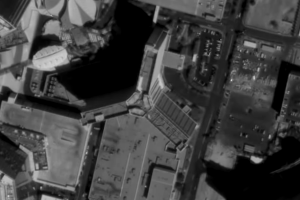
\includegraphics[height=\cropcHeight]{images/crop_comparison/crop_toit_triangle.png} &
%   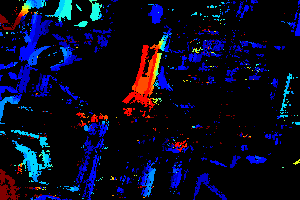
\includegraphics[height=\cropcHeight]{images/disp_confidence/crop_disparity_score_010_1stsc.png} &
%   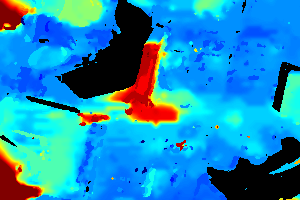
\includegraphics[height=\cropcHeight]{images/disp_confidence/crop_disparity_score_010.png}
%   \\[-0.5em]
%   \hline
  \rotatebox[origin=l]{90}{$C_d=0.05$} &
  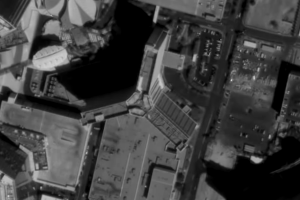
\includegraphics[height=\cropcHeight]{images/crop_comparison/crop_toit_triangle.png} &
  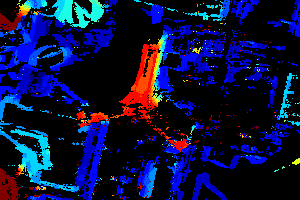
\includegraphics[height=\cropcHeight]{images/disp_confidence/crop_disparity_score_005_1stsc.png} &
  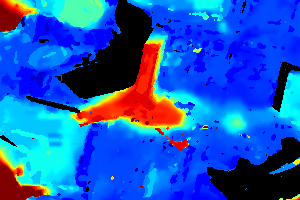
\includegraphics[height=\cropcHeight]{images/disp_confidence/crop_disparity_score_005.png}\\[-0.5em]
  \hline
  \rotatebox[origin=l]{90}{$C_d=0.02$} &
  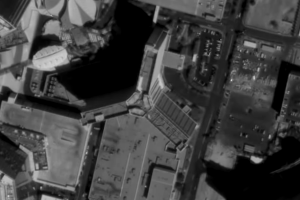
\includegraphics[height=\cropcHeight]{images/crop_comparison/crop_toit_triangle.png} &
  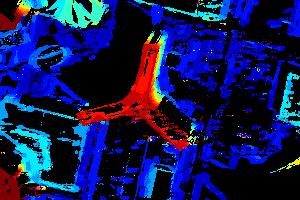
\includegraphics[height=\cropcHeight]{images/disp_confidence/crop_disparity_score_002_1stsc.png} &
  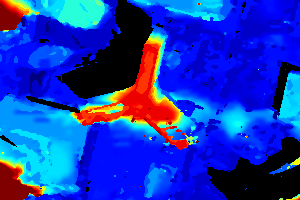
\includegraphics[height=\cropcHeight]{images/disp_confidence/crop_disparity_score_002.png}\\[-0.5em]
  \hline
  \rotatebox[origin=l]{90}{$C_d=0.01$} &
  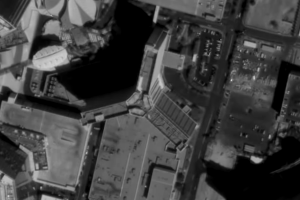
\includegraphics[height=\cropcHeight]{images/crop_comparison/crop_toit_triangle.png} &
  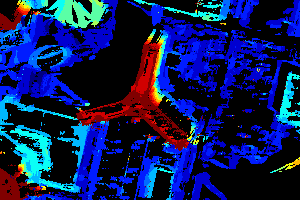
\includegraphics[height=\cropcHeight]{images/disp_confidence/crop_disparity_score_001_1stsc.png} &
  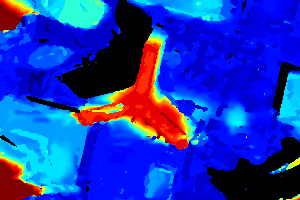
\includegraphics[height=\cropcHeight]{images/disp_confidence/crop_disparity_score_001.png}\\[-0.5em]
  \hline
  \rotatebox[origin=l]{90}{Not using $C_d$} &
  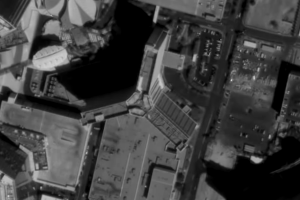
\includegraphics[height=\cropcHeight]{images/crop_comparison/crop_toit_triangle.png} &
  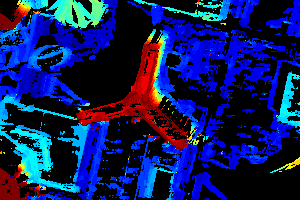
\includegraphics[height=\cropcHeight]{images/disp_confidence/crop_disparity_score_000_1stsc.png} & 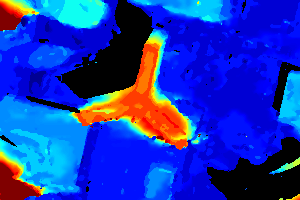
\includegraphics[height=\cropcHeight]{images/disp_confidence/crop_disparity_score_000.png}\\[-0.5em]
  \hline
  & Original & 1st scale & Result \\ \hline
 \end{tabular}
 \caption{Comparison of the results by using $C_d > 0.05,\, 0.02, \, 0.01$ and not using $C_d$ (the value used in \cite{art:kim13:lfields} is $C_d > 0.1$), on SkysatLR18 $[120]$, frame $50$. We represent the results of the first scale disparity computation ($p=0$) and the final depth map after fine-to-coarse (right). The computation times were respectively $3148$, $1878$, $1462$ and $448$ seconds.} %  ($4511$ for $C_d > 0.1$
 \label{fig:c_d_comparison}
\end{figure}


\subsection{Validation on the original dataset} 


We perform the depth estimation on one of the original datasets of Kim et al. (MansionLR) and compare our disparity map to theirs. The results are presented in Figure \ref{fig:comparison_kim}. 

As expected, our results are less precise, noticeably behind the tree (that is partially merged with the wall behind it). This can be explained by the fact that we used images of 8 MP (compared to 19 MP) and did not implement the conservative criterion $C_d$ on disparity confidence (that result in more artefacts in the final estimation). The results are quite similar on other zones: the main structures seem correctly detected and estimated, especially the foliage at the right, the tree branch silhouettes in the center, the barrier at the front and the flat surfaces on the mansion wall. This validates the pertinence and efficiency of the fine-to-coarse approach.


\begin{figure}[ht]
 \centering
 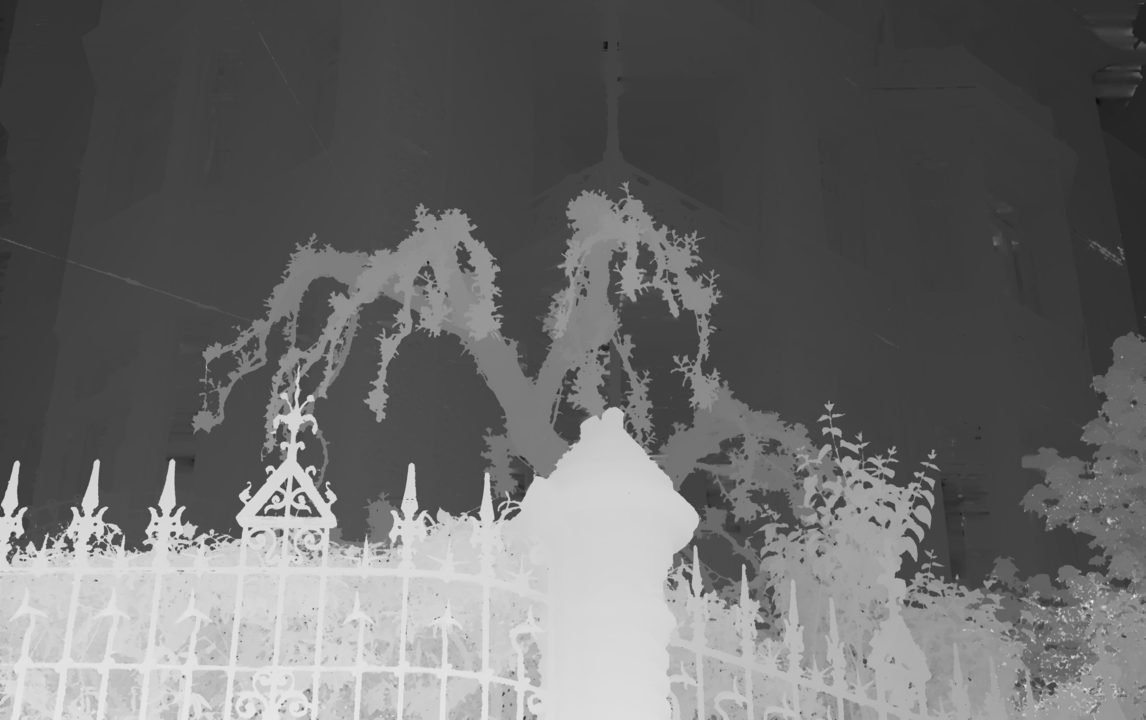
\includegraphics[width=0.7\textwidth]{images/mansion_kim_resized.png}\\
 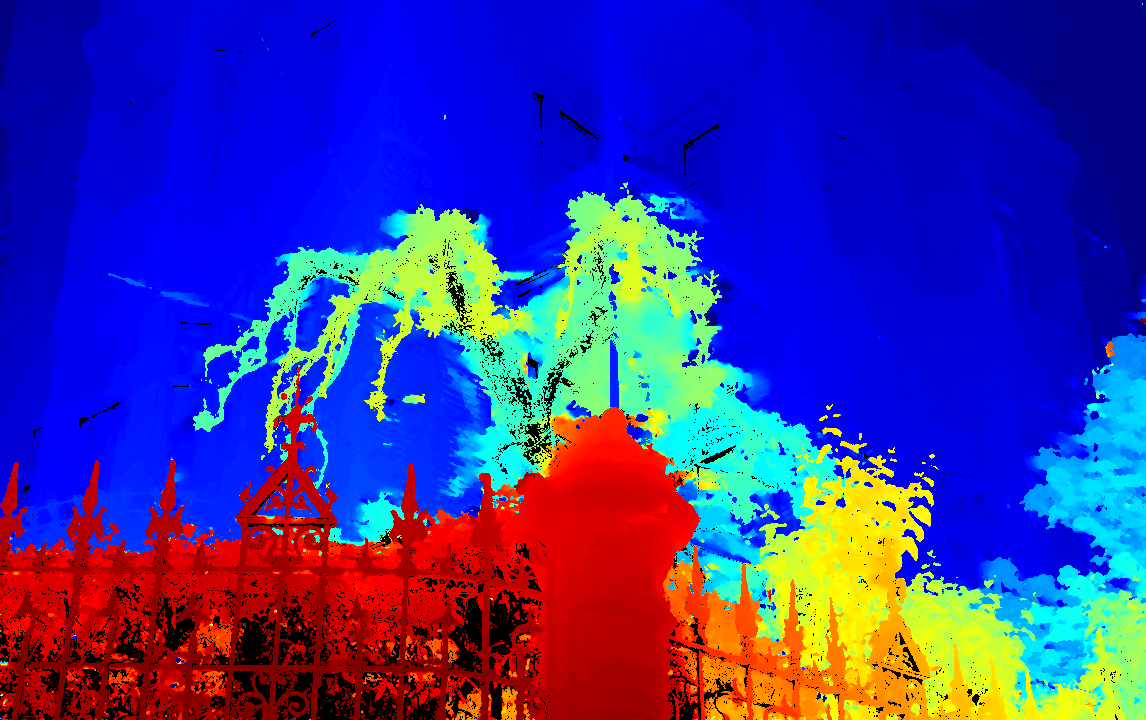
\includegraphics[width=0.7\textwidth]{images/MansionLR_240/1521776307225_dmap_050.png}
 \caption{Comparison of the results of Kim et al. in \cite{art:kim13:lfields} (top, computed using high definition images) and ours (bottom, computed with MansionLS, with $d=0:4$ $[240]$). We cut the shadows, thus the dark zones.}
 \label{fig:comparison_kim}
\end{figure}



\subsection{Influence of the resolution}


We investigate the influence of the resolution of the images on the diparity maps by using the same dataset Skysat**18 with a low resolution of $720\times 1146$ (SkysatLR18) and a high resolution of $1080\times 1920$ (SkysatHR18). We compute the disparity estimations on the same frame for these datasets in order to evaluate the influence of the higher resolution of SkysatHR18. The results are presented in Figure \ref{fig:influenceres} and close-ups are presented in Figure \ref{fig:comparison_details}. 


The disparity map computed with HR18 are noticeably more detailed for the Cross roof and the Square roof, with details being sharper and more precise. However, the results seem less accurate with HR18 than LR18 on the Triangle roof, where the fine-to-coarse approach fails to fill the bottom-right corner of the building. We assume that this is due to the fact that the corner of the roof would be merged with the texture of the side of the building in the coarser scales.


Overall the resolution seems to have a significative influence on the precision of the results. It should be noted that the computational burden is also significantly higher ($804$ seconds for LR18 $[240]$, $2888$ seconds for HR18 $[240]$).


\subsection{Influence of the slope amplitude} 


We investigate the performance of the algorithm with very small slopes with a sequence of Skysat with slower variations (SkysatLR01). A sample EPI is presented in Figure \ref{fig:epi:skysat1}. This example is harder since the variations are mostly under the scale of a pixel. We ran the algorithm with a choice of $d_{\min} = -0.5$ to $d_{\max} = 0.5$ and $120$ steps. Some results are presented in Figure \ref{fig:skysatlr01:candidated} and close-ups are presented in Figure \ref{fig:comparison_details}. These results are quite satisfactory given the small slopes to be measured, but show globally some underestimated slopes on the top of the buildings. We assume these are due to the fact that the disparities are harder to be estimated when undersampling - these may be improved by using better interpolation formulae in the algorithm, or dilate the $u$ axis using a good interpolation method as a preprocessing step.


\begin{figure}[ht]
  \centering
  \includegraphics[width=\epiWidth\textwidth]{images/1521592293547_1st.png}\\
  \includegraphics[width=\epiWidth\textwidth]{images/1521592293547_epi.png}
  \caption{Sample EPI from the Skysat sequence with slow variations.}
  \label{fig:epi:skysat1}
\end{figure}



\subsection{Influence of the candidate set of disparities}


We compare the results for the same frames of the same datasets with a number of $120$ and $240$ candidate $d$'s between the same bounds to evaluate the influence of the set of candidates on the results. The results are presented in Figures \ref{fig:skysatlr18:candidated}, \ref{fig:skysatlr01:candidated} and \ref{fig:mansionlr:candidated}. Close-ups are presented in Figure \ref{fig:comparison_details}.


On the MansionLR dataset (Figure \ref{fig:mansionlr:candidated}), the difference is minimal with almost no visible change between the simulations. On SkysatLR18 (Figure \ref{fig:skysatlr18:candidated}), we note some difference in the details of some roofs: for instance, the Square roof is noticeably more detailed in LR18[240] than in LR18[120]. These observations are also true on SkysatLR01 (Figure \ref{fig:skysatlr01:candidated}) in which the details are more visible on the Square roof and the Cross roof.


Overall, a more dense set of candidate disparities help in sharpening the details of the disparity maps. The computational burden is however linear in the number of candidates ($448$ seconds for LR18 $[120]$, $804$ seconds for LR18 $[240]$).


\clearpage
\begin{figure}[ht]
 \centering
 \includegraphics[height=8cm]{images/SkysatLR18_240_img/1521805051081_dmap_050.png}\hspace{-0.28em}
 \includegraphics[height=8cm]{images/SkysatHR18_240/1521744514157_dmap_050.png}\\
 \vspace{1em}
 \includegraphics[height=8cm]{images/SkysatLR18_240_img/1521805051081_dmap_025.png}\hspace{-0.28em}
 \includegraphics[height=8cm]{images/SkysatHR18_240/1521744514157_dmap_025.png}
 \caption{Influence of the resolution of the images. Original frame (left) SkysatLR18 $-1:4$ $[120]$ (middle) and SkysatHR18 $-1:4$ $[240]$ (right). Frame $50$ (top) and $25$ (bottom).}
 \label{fig:influenceres}
\end{figure}


\begin{figure}[ht]
 \centering
 \includegraphics[height=8cm]{images/SkysatLR18_120/1521739947374_dmap_050.png}\hspace{-0.28em}
 \includegraphics[height=8cm]{images/SkysatLR18_240/1521741442733_dmap_050.png}\\
 \vspace{1em}
 \includegraphics[height=8cm]{images/SkysatLR18_120/1521739947374_dmap_025.png}\hspace{-0.28em}
 \includegraphics[height=8cm]{images/SkysatLR18_240/1521741442733_dmap_025.png}
 \caption{Influence of the candidate disparities. SkysatLR18, original frame (left) $-1:4$ $[120]$ (middle) and $-1:4$ $[240]$ (right). Frame $50$ (top) and $25$ (bottom).}
 \label{fig:skysatlr18:candidated}
\end{figure}


\begin{figure}[ht]
 \centering
 \includegraphics[height=8cm]{images/SkysatLR01_120/1521737975374_dmap_050.png}\hspace{-0.28em}
 \includegraphics[height=8cm]{images/SkysatLR01_240/1521738847855_dmap_050.png}\\
 \vspace{1em}
 \includegraphics[height=8cm]{images/SkysatLR01_120/1521737975374_dmap_025.png}\hspace{-0.28em}
 \includegraphics[height=8cm]{images/SkysatLR01_240/1521738847855_dmap_025.png}
 \caption{Influence of the candidate disparities. SkysatLR01, original frame (left) $-1:4$ $[120]$ (middle) and $-1:4$ $[240]$ (right). Frame $50$ (top) and $25$ (bottom).}
 \label{fig:skysatlr01:candidated}
\end{figure}


\begin{figure}[ht]
 \centering
 \includegraphics[width=0.45\textwidth]{images/MansionLR_120/1521751973001_dmap_050.png}\hspace{1em}
 \includegraphics[width=0.45\textwidth]{images/MansionLR_120/1521751973001_dmap_025.png}\\
 \vspace{-0.1em}
 \includegraphics[width=0.45\textwidth]{images/MansionLR_240/1521776307225_dmap_050.png}\hspace{1em}
 \includegraphics[width=0.45\textwidth]{images/MansionLR_240/1521776307225_dmap_025.png}
 \caption{Influence of the candidate disparities. MansionLR, original frame (top) $0:4$ $[120]$ (middle) and $0:4$ $[240]$ (bottom). Frame $50$ (left) and $25$ (right).}
 \label{fig:mansionlr:candidated}
\end{figure}


\begin{figure}[ht]
 \centering
 \begin{tabular}{|c||c|c|c|}
 \hline
  \rotatebox[origin=l]{90}{LR01[120]} & 
  \includegraphics[height=\cropcHeight]{images/crop_comparison/SkysatLR01_crop_toit_120.png} &
  \includegraphics[height=\cropcHeight]{images/crop_comparison/SkysatLR01_crop_carre_120.png} &
  \includegraphics[height=\cropcHeight]{images/crop_comparison/SkysatLR01_crop_triangle_120.png}\\[-0.5em]
  \hline
  \rotatebox[origin=l]{90}{LR01[240]} &
  \includegraphics[height=\cropcHeight]{images/crop_comparison/SkysatLR01_crop_toit_240.png} &
  \includegraphics[height=\cropcHeight]{images/crop_comparison/SkysatLR01_crop_carre_240.png} &
  \includegraphics[height=\cropcHeight]{images/crop_comparison/SkysatLR01_crop_triangle_240.png}\\[-0.5em]
  \hline
  \rotatebox[origin=l]{90}{LR18[120]} &
  \includegraphics[height=\cropcHeight]{images/crop_comparison/SkysatLR18_crop_toit_120.png} &
  \includegraphics[height=\cropcHeight]{images/crop_comparison/SkysatLR18_crop_carre_120.png} &
  \includegraphics[height=\cropcHeight]{images/crop_comparison/SkysatLR18_crop_triangle_120.png}\\[-0.5em]
  \hline
  \rotatebox[origin=l]{90}{LR18[240]} &
  \includegraphics[height=\cropcHeight]{images/crop_comparison/SkysatLR18_crop_toit_240.png} &
  \includegraphics[height=\cropcHeight]{images/crop_comparison/SkysatLR18_crop_carre_240.png} &
  \includegraphics[height=\cropcHeight]{images/crop_comparison/SkysatLR18_crop_triangle_240.png}\\[-0.5em]
  \hline
  \rotatebox[origin=l]{90}{HR18[120]} &
  \includegraphics[height=\cropcHeight]{images/crop_comparison/SkysatHR18_crop_toit_120.png} &
  \includegraphics[height=\cropcHeight]{images/crop_comparison/SkysatHR18_crop_carre_120.png} &
  \includegraphics[height=\cropcHeight]{images/crop_comparison/SkysatHR18_crop_triangle_120.png}\\[-0.5em]
  \hline
  \rotatebox[origin=l]{90}{HR18[240]} &
  \includegraphics[height=\cropcHeight]{images/crop_comparison/SkysatHR18_crop_toit_240.png} &
  \includegraphics[height=\cropcHeight]{images/crop_comparison/SkysatHR18_crop_carre_240.png} &
  \includegraphics[height=\cropcHeight]{images/crop_comparison/SkysatHR18_crop_triangle_240.png}\\[-0.5em]
  \hline
  \rotatebox[origin=l]{90}{Frame} & 
  \includegraphics[height=\cropcHeight]{images/crop_comparison/crop_toit_cross.png} &
  \includegraphics[height=\cropcHeight]{images/crop_comparison/crop_toit_square.png} &
  \includegraphics[height=\cropcHeight]{images/crop_comparison/crop_toit_triangle.png}\\[-0.5em]
  \hline
  & Cross roof & Square roof & Triangle roof \\ \hline
 \end{tabular}
 \caption{Close-up comparison between the different tests on frame $50$ for each Skysat dataset and $[\text{number of disparity candidates}]$ (it should be noted that these are different, yet comparable, for SkysatLR01) for different zones of the disparity maps.}
 \label{fig:comparison_details}
\end{figure}


\clearpage
\subsection{Limitations} 


We notice some new issues in the particular case of satellite imagery. The best estimates are made for frames near $\widehat{s} = \dim s / 2$ as the propagation process might end up perturbating the estimates since we did not use the conservative criterion $C_d$ that would reject low confidence $d$ estimates. Moreover, satellite images are subject to perturbations such as:
\begin{itemize}
 \item Objects appearing and disappearing (such as the walls of buildings), moving objects like cars (which are likely to persist in several frames, or which are numerous in the same regions and will be merged in the same EPI disparity line).
 \item Objects changing shape (for instance, the walls of a building are likely to change shape due to perspective effects) which disparities vary quickly spatially and would be likely to be merged by the fine-to-coarse approach.
 \item Global changes in illumination conditions. This happens in some frames in the Skysat dataset but seems to have a low impact on the results and can be corrected with some preprocessing equalization.
 \item Shadows will be interpreted as rough confident edges, but are not textured, so their depth estimates will be flawed. We thus decided to remove these areas as described in Subsection \ref{subsec:dataset_params}.
 \item Tricky surfaces such as reflective surfaces (the glass surfaces on buildings) will be misinterpreted since they have the same texture as the ground and could have a disparity dependant on the viewpoint of the camera.
\end{itemize}


\begin{figure}[ht]
 \centering
 \begin{tabular}{|c||c|c|c|}
 \hline
 \rotatebox[origin=l]{90}{EPI} & 
  \includegraphics[height=\cropcHeight]{images/detail_closeup/crop_detail_epi.png} &
  \includegraphics[height=\cropcHeight]{images/detail_closeup/crop_flash_epi.png} &
  \includegraphics[height=\cropcHeight]{images/detail_closeup/crop_car_epi.png}
   \\[-0.5em]
  \hline
  \rotatebox[origin=l]{90}{Frame} & 
  \includegraphics[height=\cropcHeight]{images/detail_closeup/crop_detail.png} &
  \includegraphics[height=\cropcHeight]{images/detail_closeup/crop_flash.png} &
  \includegraphics[height=\cropcHeight]{images/detail_closeup/crop_car.png}
   \\[-0.5em]
  \hline
  \rotatebox[origin=l]{90}{LR18 $[120]$} &
  \includegraphics[height=\cropcHeight]{images/detail_closeup/crop_detail_LR18_240.png} &
  \includegraphics[height=\cropcHeight]{images/detail_closeup/crop_flash_SkysatLR18_240.png} &
  \includegraphics[height=\cropcHeight]{images/detail_closeup/crop_car_SkysatLR18_240.png}
  \\[-0.5em]
  \hline
  & Mirror reflects & Specular reflections & Moving objects \\ \hline
 \end{tabular}
 \caption{Limitations: mirror reflects on building sides, specular reflections, moving objets like cars.}
 \label{fig:limitations}
\end{figure}


\clearpage
\section{Conclusion and perspectives}


In this project, we implemented a method of Kim et al. in order to estimate disparity maps (and thus depth maps) from sequences of images taken along a linear path (light fields). The case of rectified satellite images corresponds to the specific case in which the ground is thrown back to infinity.


We tested the method on videos of Las Vegas taken by Skysat. It appears that the results are quite satisfactory, and that indeed a higher resolution, more pronounced slopes and more candidate disparities increase the precision of the results, often with some larger computational cost. 


Some leads to improve further the results are presented below:
\begin{enumerate}
 \item As described earlier, contrary to the method presented in \cite{art:kim13:lfields}, we did not use a conservative confidence criterion to reject $d$'s with a low confidence score, i.e. we assumed that any point with a high edge confidence score $C_e$ would have a high confidence score $C_d$. The reason was that $C_d$ seemed too conservative for our satellite images. As an improvement, one could for instance consider some other criterion like
 \begin{align}
  C_l &= \frac{\sum C_e(\mathbf{r}) K(\mathbf{r} - \overline{\mathbf{r}})}{\sum K(\mathbf{r} - \overline{\mathbf{r}})}
 \end{align}
 that would be less conservative and yet ensure that a line is indeed well defined in the EPI.
 \item As a way to keep as much information as possible during the downsampling step, one could consider for instance adding a supplementary channel to the EPIs that would contain the derivative of the image. This method was successfully applied for instance in the context of inpaining (see \cite{art:liu:deriv} and \cite{art:newson:deriv}).
 \item Contrary to the method of \cite{art:kim13:lfields}, we did not implement our algorithm on GPU. It could be possible to adapt our code with some adjustments in the interpolation scheme.
 \item In order to avoid the issue of slopes being too small to be correctly estimated, one could use other interpolation methods (here we only used a linear interpolation) or equivalently dilate the spatial dimension $u$ during preprocessing using a good interpolation method.
\end{enumerate}



% \section{Choice of the article and objective}
% 
% 
% We first investigated two different articles that describe two different methods for estimating depths maps from videos.
% \begin{itemize}
%  \item \cite{art:perez13:tvl1} describes an algorithm that estimates the optical flow given two images using a global optimization scheme minimizing a data attachment term and a regularization using the total variation of the flow. The idea is that the brightness $I$ of single points along their trajectories should be constant in time, leading to the optical flow constraint equation
%  \[ \nabla I \cdot \vect{u} + \Dpar{I}{t} = 0 \]
%  where $\vect{u}$ is the optical flow (the velocity vector field). The article then introduces a regularization on $\vect{u}$ (its total variation) and reformulates the problem in order to adapt to discrete sequences of images so that the attachent term consists in minimizing some $L^1$ term. In order to solve the subsequent global optimization problem, the authors propose a numerical scheme based on alternate optimization scheme. Finally, the authors investigate the influence of the several parameters of the algorithm -- noticeably the weight $\lambda$ of the data attachment term -- on the precision of the estimation of the optical flow and the sensitivity to noise.
%  
%  In our case, the optical flow computed with this algorithm could be interpreted as some disparity measurement. An interesting point is that the computation of the optical flow can be done on any pair of images, even if not rectified.
%  
%  \item \cite{art:kim13:lfields} describes a method for computing precise and exhaustive depth maps using ``light fields'', that is a dense set of images captures along a linear path. By concatenating one line of the rectified images together, one obtains an ``epipolar-plane image'' (EPI), in which a single scene point appears as a linear trace which slope is related to its distance to the camera. Thus, by estimating these slopes, one can reconstruct the depth of each point of the scene.
%  
%  The authors use very high definition images, so that the article includes several implementation details in order to ensure computational feasibility, both in terms of space (sparse representation of light fields) and computational power. For instance, they prefer local optimization near object boundaries and propagation to nearby areas in a fine-to-coarse approach to global optimization on the whole image. In the end, the method seems relatively fast, precise and robust to inconsistencies and outliers like noise or temporary occlusions.
% \end{itemize}


% We chose to work on the latter article. The objective of the project is then to implement the method presented by Kim et al. in \cite{art:kim13:lfields} and investigate how it performs with videos taken from SkySat. We will first investigate the case in which the images from the video are pre-rectified. Then we will investigate more complicated situations, for instance increasing the density of the images and considering non-pre-rectified sequences.


\bibliographystyle{plain}
\bibliography{bibliography}


\appendix
\section{Implementation details}


We implemented our algorithm using \verb#C++# and \verb#OpenCV#. The Doxygen documentation for the project can be found here:
\begin{center}
 \url{https://14chanwa.github.io/remotesensingProject/}
\end{center}


\subsection{Structure of the project}


The project is organized in headers in the folder \verb#include/# and source files in the folder \verb#src/#. Most of the low-level functions are defined in the files \verb#rslf_depth_computation_core.hpp# and \verb#rslf_fine_to_coarse_core.hpp# and the high-level instances are defined in \verb#rslf_depth_computation.hpp# and \verb#rslf_fine_to_coarse.hpp#.


\begin{figure}[ht]
  \centering
  \includegraphics[height=9.5cm, trim=0cm 1cm 0cm 1cm, clip]{drawings/rslf_8hpp__incl.pdf}
  \caption{Header inclusion dependency tree}
  \label{fig:header:dependancy}
\end{figure}


As described in the \verb#CMakeLists.txt# file, the program will be compiled under the form of a library and tests using functions from this library. In order to use the algorithms, we only have to add a \verb#.cpp# file in the \verb#tests/# folder and re-run \verb#CMake#. In order to get the right paths for the existing tests, we can run the following commands from the folder containing \verb#README.md#:
\begin{verbatim}
mkdir build
cd build
cmake ../RSLightFields
make
\end{verbatim}


As for global aliases, \verb#rslf::Mat# is \verb#cv::Mat# and \verb#rslf::Vec<T># is \verb#std::vector<T>#. \verb#rslf::Mat# structures are bi-dimensional. A tri-dimensional structure will be stored using \verb#rslf::Vec<rslf::Mat>#.



\subsection{High-level classes}


In order to run the algorithm, one can use the high-level classes as presented in Figure \ref{code:mwe:ftc}.

\begin{figure}[ht]
\begin{lstlisting}
#include <rslf.hpp>
#include <opencv2/core/core.hpp>

using namespace rslf; // Library namespace
int main() {
    // Load images (assume the folder contains only the images, in alphanumerical order)
    // The flag should be set according to the input images: float is CV_LOAD_IMAGE_UNCHANGED, other files are either CV_LOAD_IMAGE_COLOR or CV_LOAD_IMAGE_GRAYSCALE
    Vec<Mat> list_mat = read_imgs_from_folder("path_to_folder", "extension", CV_LOAD_IMAGE_UNCHANGED); 
    Vec<Mat> epis = build_epis_from_imgs(list_mat);
    float d_min = 0.0;
    float d_max = 4.0;
    int dim_d = 120;
    // Use FineToCoarse_1ch for monochromatic, FineToCoarse_3ch for RGB images 
    FineToCoarse_1ch fine_to_coarse(epis, d_min, d_max, dim_d);
    fine_to_coarse.run();
    Vec<Mat> out_map_s_v_u_;
    Vec<Mat> out_validity_s_v_u_;
    fine_to_coarse.get_results(out_map_s_v_u_, out_validity_s_v_u_);
    // ...
    return 0;
}
\end{lstlisting}
\caption{Minimal working example for fine-to-coarse}
\label{code:mwe:ftc}
\end{figure}


We included several high-level classes that perform different operations on EPIs:
\begin{itemize}
 \item \verb#FineToCoarse# executes the entire pipeline described in this document.
 \item \verb#Depth1DComputer# computes only the disparity map for $\widehat{s} = s_{\max}/2$ one one given EPI (i.e. $v$ is fixed).
 \item \verb#Depth1DComputer_pile# takes a pile of EPIs (a pile of $(s, u)$ images along the dimension $v$) and computes a disparity map for $\widehat{s} = s_{\max}/2$ for each $v$.
 \item \verb#Depth2DComputer# takes a pile of EPIs and compute the disparity maps for all $v$ and all $s$ using the disparity propagation process.
\end{itemize}
These are template classes which internal structures depend on the number of channels of the image. Aliases are defined such as \verb#FineToCoarse_1ch#, \verb#Depth2DComputer_3ch#... are defined for convenience. The algorithm only supports monochromatic and RGB images.


\subsection{Low-level functions and complexity}


\paragraph{Depth computation} The main computations are handled by the low-level functions written in the file \verb#rslf_depth_computation_core.hpp#.
\begin{enumerate}
 \item \verb#compute_1D_edge_confidence# will compute $C_e$ for a single line $s$ of a single EPI $v$. The rough complexity is $\grandO{u}$.
 \item \verb#compute_1D_depth_epi# will compute the slope estimation for a single line $s$ of a single EPI $v$. The rough complexity is $\grandO{ud}$.
 \item \verb#compute_1D_edge_confidence_pile# will call \verb#compute_1D_edge_confidence# on the single line $s$ of every EPI $v$ (given the corresponding vector of EPIs). The rough complexity is $\grandO{vu}$.
 \item \verb#compute_1D_depth_epi_pile# will call \verb#compute_1D_depth_epi# on the single line $s$ of every EPI $v$ (given the corresponding vector of EPIs). The rough complexity is $\grandO{vud}$.
 \item \verb#compute_2D_edge_confidence# will call \verb#compute_1D_edge_confidence_pile# on every line $s$ so that every point $(s, v, u)$ is given a score $C_e$. The rough complexity is $\grandO{svu}$. This step proves very fast in practice.
 \item \verb#compute_2D_depth_epi# will call \verb#compute_1D_edge_confidence_pile# on every line $s$ so that every point $(s, v, u)$ with a sufficient confidence score will be given a disparity value. The rough empirical complexity is $\grandO{vud}$, as the propagation process significantly reduces the complexity in $v$, $u$, $d$ at a given $s$ after the first iteration on $\widehat{s}=s_{\max}/2$.
\end{enumerate}
Note that these are template functions that depend on the number of channel of the input EPIs. The functions for RGB images are significantly more intensive than the functions for monochromatic images, as shown by the runtimes in Table \ref{table:tests}.

\paragraph{Fine to coarse}
The implementation makes use of the high-level classes for depth computation. The algorithm will run on downsampled images $u \leftarrow u/2$, $v \leftarrow v/2$ at each step, so that the overall empirical complexity will still be $\grandO{vud}$.


% C++


% Diagramme de classes


% Fonctions et minimal working example


\end{document}